% $Id: template.tex 11 2007-04-03 22:25:53Z jpeltier $

\documentclass{vgtc}                          % final (conference style)
%\documentclass[review]{vgtc}                 % review
%\documentclass[widereview]{vgtc}             % wide-spaced review
%\documentclass[preprint]{vgtc}               % preprint
%\documentclass[electronic]{vgtc}             % electronic version

%% Uncomment one of the lines above depending on where your paper is
%% in the conference process. ``review'' and ``widereview'' are for review
%% submission, ``preprint'' is for pre-publication, and the final version
%% doesn't use a specific qualifier. Further, ``electronic'' includes
%% hyperreferences for more convenient online viewing.

%% Please use one of the ``review'' options in combination with the
%% assigned online id (see below) ONLY if your paper uses a double blind
%% review process. Some conferences, like IEEE Vis and InfoVis, have NOT
%% in the past.

%% Figures should be in CMYK or Grey scale format, otherwise, colour 
%% shifting may occur during the printing process.

%% These few lines make a distinction between latex and pdflatex calls and they
%% bring in essential packages for graphics and font handling.
%% Note that due to the \DeclareGraphicsExtensions{} call it is no longer necessary
%% to provide the the path and extension of a graphics file:
%% \includegraphics{diamondrule} is completely sufficient.
%%
\ifpdf%                                % if we use pdflatex
  \pdfoutput=1\relax                   % create PDFs from pdfLaTeX
  \pdfcompresslevel=9                  % PDF Compression
  \pdfoptionpdfminorversion=7          % create PDF 1.7
  \ExecuteOptions{pdftex}
  \usepackage{graphicx}                % allow us to embed graphics files
  \DeclareGraphicsExtensions{.pdf,.png,.jpg,.jpeg} % for pdflatex we expect .pdf, .png, or .jpg files
\else%                                 % else we use pure latex
  \ExecuteOptions{dvips}
  \usepackage{graphicx}                % allow us to embed graphics files
  \DeclareGraphicsExtensions{.eps}     % for pure latex we expect eps files
\fi%

%% it is recomended to use ``\autoref{sec:bla}'' instead of ``Fig.~\ref{sec:bla}''
\graphicspath{{figures/}{pictures/}{images/}{./}} % where to search for the images

\usepackage{microtype}                 % use micro-typography (slightly more compact, better to read)
\PassOptionsToPackage{warn}{textcomp}  % to address font issues with \textrightarrow
\usepackage{textcomp}                  % use better special symbols
\usepackage{mathptmx}                  % use matching math font
\usepackage{times}                     % we use Times as the main font
\renewcommand*\ttdefault{txtt}         % a nicer typewriter font
\usepackage{cite}                      % needed to automatically sort the references
% \usepackage{tabu}                      % only used for the table example
% \usepackage{booktabs}                  % only used for the table example
%% We encourage the use of mathptmx for consistent usage of times font
%% throughout the proceedings. However, if you encounter conflicts
%% with other math-related packages, you may want to disable it.
% * <jchae@purdue.edu> 2017-07-05T19:53:15.710Z:
%
% ^.

\let\svthefootnote\thefootnote

%% If you are submitting a paper to a conference for review with a double
%% blind reviewing process, please replace the value ``0'' below with your
%% OnlineID. Otherwise, you may safely leave it at ``0''.
\onlineid{0}

%% declare the category of your paper, only shown in review mode
\vgtccategory{Research}

%% allow for this line if you want the electronic option to work properly
\vgtcinsertpkg

%% In preprint mode you may define your own headline.
%\preprinttext{To appear in an IEEE VGTC sponsored conference.}

%% Paper title.

\title{Visualization for Classification in Deep Neural Networks}

%% This is how authors are specified in the conference style

%% Author and Affiliation (single author).
%%\author{Roy G. Biv\thanks{e-mail: roy.g.biv@aol.com}}
%%\affiliation{\scriptsize Allied Widgets Research}

%% Author and Affiliation (multiple authors with single affiliations).
%%\author{Roy G. Biv\thanks{e-mail: roy.g.biv@aol.com} %
%%\and Ed Grimley\thanks{e-mail:ed.grimley@aol.com} %
%%\and Martha Stewart\thanks{e-mail:martha.stewart@marthastewart.com}}
%%\affiliation{\scriptsize Martha Stewart Enterprises \\ Microsoft Research}

%% Author and Affiliation (multiple authors with multiple affiliations)
\author{Junghoon Chae\thanks{e-mail: chaej@ornl.gov}\qquad Shang Gao\thanks{e-mail:gaos@ornl.gov}\qquad Arvind Ramanthan\thanks{e-mail:ramanathana@ornl.gov}\qquad Chad Steed\thanks{e-mail:csteed@ornl.gov}\qquad Georgia D. Tourassi\thanks{e-mail:tourassig@ornl.gov} \\ %
        \scriptsize Oak Ridge National Laboratory %
%      \parbox{1.4in}{\scriptsize \centering Martha Stewart Enterprises \\ Microsoft Research}
}


%% A teaser figure can be included as follows, but is not recommended since
%% the space is now taken up by a full width abstract.
\teaser{
 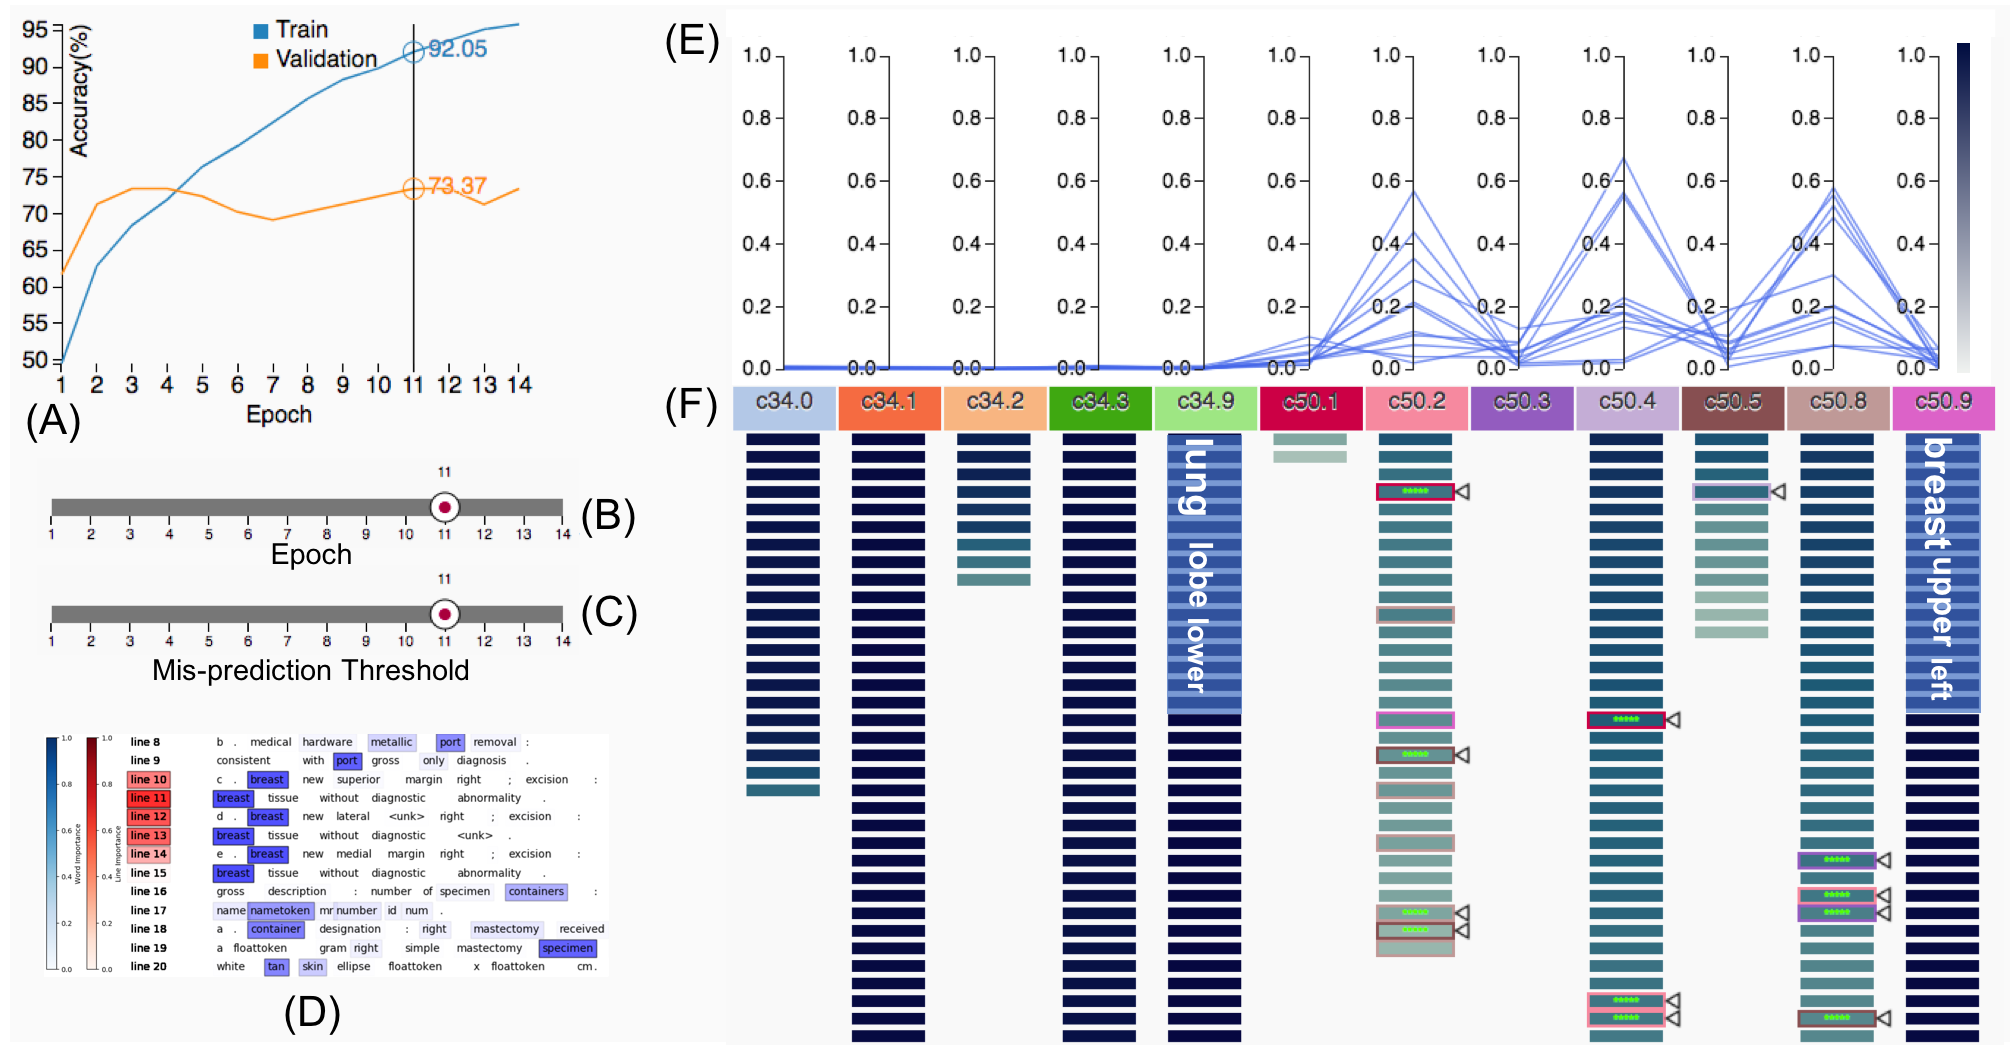
\includegraphics[width=0.98\linewidth]{teaser_v2}
 \caption{A visual analytics tool to understand classification results and suggest potential directions during the development of a Deep Neural Networks model.}
 \label{fig:teaser}
}

%% Abstract section.
\abstract{
% Classification is one of the major tasks in a wide range of data analysis tasks.
Recently, the techniques based on Deep Neural Networks (DNNs) have achieved a great performance in classification tasks in a wide range of applications, such as image recognition and natural language processing.
However, DNN developers face a lot of trial and error during the development process and spend their efforts in developing their network model through analyzing and understanding the classification results.
As such, tools are needed that help the developers not only understand the results, but also suggest the ways to improve their model.
In this paper, we propose a visual analytics tool for visualizing the classification results during the iterative development pipeline of a DNN model.
Our tool enables exploring the classification results from any type of neural network models, identifying misclassified samples, examining the predicted score distributions of samples, and showing how the outcomes progressively change during the training process.
% Our visual analytics approach enables exploring the classification results from any type of neural network models, examining the predicted score distributions for each sample data, and showing how the results change progressively during the training process in order to understand, diagnose, and improve the network models.
% In this paper, however, we focus on the document classification by a Hierarchical Attention Network (HAN) model based on a Recurrent Neural Network (RNN) ~\cite{yang2016hierarchical} as a case study.
} % end of abstract

%% ACM Computing Classification System (CCS). 
%% See <http://www.acm.org/class/1998/> for details.
%% The ``\CCScat'' command takes four arguments.

\CCScatlist{ 
  Visualization, classification, deep neural networks
}

% H.5.2 [Information Interfaces and Presenta- tion]: User Interfaces—GUI; H.3.3 [Information Storage and Retrieval]: Information Search and Retrieval—Information filtering, relevance feedback

%% Copyright space is enabled by default as required by guidelines.
%% It is disabled by the 'review' option or via the following command:
% \nocopyrightspace

%%%%%%%%%%%%%%%%%%%%%%%%%%%%%%%%%%%%%%%%%%%%%%%%%%%%%%%%%%%%%%%%
%%%%%%%%%%%%%%%%%%%%%% START OF THE PAPER %%%%%%%%%%%%%%%%%%%%%%
%%%%%%%%%%%%%%%%%%%%%%%%%%%%%%%%%%%%%%%%%%%%%%%%%%%%%%%%%%%%%%%%%

\begin{document}

%% The ``\maketitle'' command must be the first command after the
%% ``\begin{document}'' command. It prepares and prints the title block.

%% the only exception to this rule is the \firstsection command
\firstsection{Introduction}
\maketitle
%% \section{Introduction} %for journal use above \firstsection{..} instead
Classification is one of the major tasks in a wide range of data analysis tasks.
Recently, the techniques based on Deep Neural Networks (DNNs) have achieved a great performance in classification tasks for a wide range of applications, such as image~\cite{krizhevsky2012imagenet}, video~\cite{karpathy2014large}, text~\cite{kim2014convolutional}, and natural language~\cite{collobert2011natural}.
However, DNN developers face a lot of trial and error to develop a satisfying DNN model.
During the trial and error process, they spend their efforts in developing their network model through analyzing and understanding intermediate experimental results.
As such, tools are needed that help them not only understand the outcomes, but also suggest the ways to improve their model.

In this paper, we propose a visual analytics tool to understand classification results and suggest potential directions during the iterative development pipeline of a DNN model.
Our visual analytics tool allows users to explore the classification results from any type of neural network models, to identify misclassified samples, to examine the predicted score distributions of samples, and to show how the outcomes progressively change during the training process.
Eventually, our visualization helps the users understand, diagnose, and improve DNN models~\cite{liu2017towards}.
Also, our visual design can be applied to a wide range of data classification tasks in deep learning.
In this paper, we focus on the task of classifying clinical pathology reports by DNNs.
This work is in progress now.
So, we focus on introducing the current system and showing preliminary results.

\let\thefootnote\relax\footnote{\tiny{This manuscript has been authored by UT-Battelle, LLC under Contract No.\ DE-AC05-00OR22725 with the U.S.\ Department of Energy. The United States Government retains and the publisher, by accepting the article for publication, acknowledges that the United States Government retains a non-exclusive, paid-up, irrevocable, worldwide license to publish or reproduce the published form of this manuscript, or allow others to do so, for United States Government purposes. The Department of Energy will provide public access to these results of federally sponsored research in accordance with the DOE Public Access Plan (http://energy.gov/downloads/doe-public-access-plan).}}

\section{Related Work}
\label{sec:related}

The technologies based on DNNs have been used widely in data science, since DNNs have shown great promise in image recognition~\cite{krizhevsky2012imagenet}.
Also, a number of researchers have proposed new models beyond the state-of-the-art techniques.
In this section we introduce some previous studies related to this work.
We discuss how visualizations have played in development of DNN models and the differences between our work and the previous work.

% \subsection{Visualization in Deep Learning}
Although DNNs make great achievements, understanding of what computations performed at intermediate layers of DNNs is still limited.
Some previous studies have developed tools that help understand the processes in DNNs through visualization techniques.
They have proved such tools can help DNN developers improve their network models~\cite{tzeng2005opening,yosinski2015understanding,liu2017towards}.
Here, we discuss the roles of visualization with regard to the following three topics:

\textbf{Understanding of the Underlying Processes in Networks:}
The most important purpose of visualizations for DNNs is to understand the underlying processes in networks.
The visualizations can be classified into two categories according to which aspects of the network are visualized: \textbf{Inner Process} and \textbf{Learned Features}.
\begin{itemize}
\item \textbf{Inner Process:}
Visualizations in this category directly represent the interactions between neurons in a network.
These visualizations enable intuitive understanding of the inner processes in the networks.
Tzeng and Ma~\cite{tzeng2005opening} employed a directed acyclic graph (DAG) to show the interactions between neurons in the three different layers: input, hidden, and output.
The visualization, however, has a visual clutter issue when handling a large number of neurons.
Liu et al.~\cite{liu2017towards} also used a similar type of visualization, but they mitigate the issue.
They clustered layers and neurons in networks, selected representative layers and neurons, and illustrated those by a hybrid visualization.
Harley~\cite{harley2015interactive} developed an interactive and intuitive visualization system for DNNs.
Given an input image drawn by an user, the visualization system shows not only the features learned by networks, but also the behavior (i.e., activation and interaction) of neurons and layers.

\item \textbf{Learned Features:}
This type of visualizations focuses on visualizing the features learned by networks rather than the behavior in networks.
Since Convolutional Neural Networks (CNNs), a specific type of DNNs, have been widely used for image classification, many visualization approaches have been proposed to understand how images are classified by CNNs~\cite{erhan2009visualizing,zeiler2014visualizing,yosinski2015understanding,nguyen2016multifaceted}.
The visualizations display synthetic images produced by gradient-based techniques including deconvolution, code inversion, activation maximization\textemdash these techniques are based on high activations (learned features) of neurons of a network.
The images (although they do not look natural) would provide insight into the network model and can suggest potential directions to improve the model.
In addition to CNNs, Recurrent Neural Networks (RNNs) are getting attention since RNNs have achieved a great performance for sequential data, such as streaming, speech, and document.
Strobelt~\cite{strobelt2016visual} proposed a visual analytics system to understand a RNN-based model, where the system helps users explore hidden states in RNNs and find similar patterns in data.
\end{itemize}

The previous studies have made great achievements and shown the importance of visualization in development of DNNs.
However, they still have limitations.
For the clustering approach, when handling a large network, finding an appropriate abstraction level of networks would be a challenge.
Also, the DAG-based visualizations have a limitation in supporting other types of networks beside CNN-based networks.
For visualizing learned features, when the number of samples and classes is huge, it would be not easy to gain insights into the networks by analyzing the learned features of every single samples.
Although our approach is close to the second category, we focus on visualizing and understanding classification results of any types of DNNs.
%We argue that after DNN developers gain insights into data and classification results, they would more effectively understand the inner processes and the learned features using the aforementioned techniques than without the initial step.

% We argue that it should be effective to improve a network model after understanding initial classification results by using a basic network model.
% For classification tasks in real industrial world applications, such as medical records, CT scan images, 2D neutron scattering images, those who develop DNNs for a specific application would be not experts in the area.
% Therefore, in the situation that DNN developers has no background knowledge about the data they are dealing with and cannot expect the output, starting with the understanding of initial classification outputs resulted by their prototype model should help them develop the model for a specific data.
% After this preceding step, they would more effectively understand the inner processes and the learned features using the aforementioned techniques than without the step.

\textbf{Visualization for Classification Result:}
Visualization enables a better understanding of the classification results of neural networks.
Especially, when handling a large size of samples, suitable visualization techniques are required.
Most techniques have used a 2D-embedding type of visualization (Figure~\ref{fig:t-sne}) to represent the classification results.
An output layer of neural networks usually produce predicted scores for each sample across all classes.
They project the prediction scores on a 2D space by dimensionality reduction techniques, such as t-SNE, PCA, etc~\cite{maaten2008visualizing,rauber2017visualizing,kahng2018activis,paiva2015approach}.
This type of visualizations has a visual clutter issue caused by the large number of data points.
If the number of classes is large, the issue will become even worse.
Also, the visualizations are not able to reveal the assigned predicted score distribution over the classes.
Our visual representation solves these issues.
Our stripe visualization has a better scalability, resolves the visual clutter issue, and effectively shows the probability distribution by integrating a parallel coordinated visualization into our tool.
Details are described in Section~\ref{sec:visualization}.
Ren et al.~\cite{ren2017squares} proposed a visualization for performance analysis in machine learning.
Their major visual metaphor and the way they use that metaphor is similar to our approach.
In this paper, our visualization tool focuses on the understanding of classification results rather than performance analysis.
Besides, we visualize how the outcome changes, which samples are continuously misclassified, and what features are learned by the neural networks as the training progress.
This provides opportunities to improve the model.

\textbf{Direct Manipulation:} Few previous studies proposed approaches that support direct manipulation of neural networks and a real-time visualization of the networks~\cite{smilkov2016direct,chung2016revacnn}.
Both Playground~\cite{smilkov2016direct} and ReVACNN~\cite{chung2016revacnn} provide similar features.
They support real-time visualization of how neural networks are trained and real-time model steering\textemdash selecting filters, adding/removing neurons/layers, and adjusting weights.
The tools help users gain an intuition about deep neural networks.
Playground, however, is designed for an educational purpose rather than real-world applications.

\begin{figure}[tb]
\centering
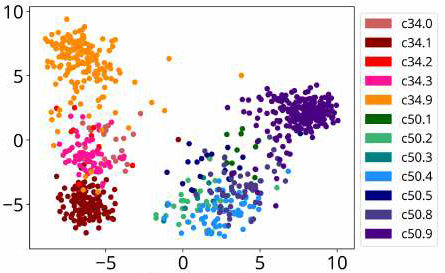
\includegraphics[width=0.7\columnwidth]{2d-embedding}
\caption{
2D-embedding of cancer pathology reports using PCA.
The colors of the points denote their classes.
%This type of visualization has limitations in understanding a classification result~\cite{rauber2017visualizing}.
}
\label{fig:t-sne}
%\vspace{-0.8cm}
\end{figure}


% \item Visualizing the Hidden Activity of Artificial Neural Networks~\cite{rauber2017visualizing}
% \item Recurrent Models of Visual Attention
% \item VISUALIZING AND UNDERSTANDING RECURRENT NETWORKS
% \item Towards Transparent AI Systems: Interpreting Visual Question Answering Models
% \item ML-o-scope: a diagnostic visualization system for deep machine learning pipelines
% \item Visualizing Deep Convolutional Neural Networks Using Natural Pre-imag
% Increase Transparency - Interpreting Black-Box Classifiers Using Instance-Level Visual Explanations

% \subsection{Visualization for Classification}

% \begin{enumerate}
% \item Modelling, Visualising and Summarising Documents with a Single Convolutional Neural Network
% \item Convolutional Neural Networks for Sentence Classification
% \item Power to the People: The Role of Humans in Interactive Machine Learning
% \item Visualizing and Understanding Neural Models in NLP
% \item Multi-task Deep Neural Networks for Automated Extraction of Primary Site and Laterality Information from Cancer Pathology Reports~\cite{yoon2016multi}
% \end{enumerate}


\section{Design Requirements}
\label{sec:design}

Our hypothesis is that the understanding of classification results can be effective to improve a neural network model.
In the real-world, the application domain for classification can be very specific, for example, medical records, CT scan images, scientific images.
In most cases, however, neural network developers would be not experts in a specific application domain.
If the model developers have no background knowledge about the data they deal with and even they cannot expect any classification outcomes, starting with the understanding of data and classification outputs using our visualization tool should help them improve their network model for a specific classification task.
Through this preceding step, they can more clearly understand the inner working and the learned features of their neural networks than without the step.

We discussed visual design requirements for understanding classification with deep learning experts many times.
We realized that they need not only basic visualizations for classification, but also specific requirements for their DNN models.
The basic visual design needs to support the following requirements: \textit{exploration of the classifications}, \textit{a summary of each class}, and \textit{a detail view of each sample}.
In addition to these basic requirements, we identified the following specific visualization requirements for supporting the aspects of DNNs.
\begin{itemize}
\item \textbf{R1: Showing training result changes as a training progressed.}
Visualization needs to allows experimenters to monitor the accuracy and outcome of a network model during its training process.
This allows to find a best performance point or stop the network from over-fitting~\cite{yeager2016effective}.
Also, the experts need to identify the misclassified or ambiguously classified samples.
\item \textbf{R2: Examining classification probability distributions.}
Neural networks usually produce score distributions over all classes.
The class with the highest score is selected as the predicted class.
It is important to visualize the score distribution.
For example, they need to see the second and third highest probability of classification of a misclassified or ambiguous data set to find possible solutions and refine their network model.
\item \textbf{R3: Revealing the features of data learned by neural networks.}
The experts want to view the learned features of each training sample.
They examine the features to discover the issues of their network model.
For example, they can recognize noise in training data that highly affects the networks and then handle the noise to refine their model.
\end{itemize}






\section{Background}
\label{sec:background}

In this work, we focus on classification of clinical pathology reports.
Clinical pathology reports contains highly valuable information.
However, many experts have manually classified the huge volume of pathology reports and extracted information from the reports.
Also, the reports are usually unstructured and have highly varied formats because they are generated from hundreds of different medical facilities and providers.

Recently, Deep Learning (DL) based approaches in Natural Language Processing (NLP) have been applied for analysis of pathology reports and health records~\cite{yoon2016multi,miotto2016deep,qiu2017deep}.
Yoon et al.~\cite{yoon2016multi} proposed a multi-task learning model to extract important keywords from cancer pathology reports.
Moitto et al.~\cite{miotto2016deep} presented clinical predictive model using a unsupervised DL to derive patient representations that improve clinical prediction and decision system.
Recurrent Neural Networks (RNNs) have achieved a great performance in NLP tasks.
Yang et al.~\cite{yang2016hierarchical} developed a Hierarchical Attention Network (HAN) which is based on RNNs.
They designed the networks to capture a hierarchical structure of documents (words form sentences, sentences form a document).
HAN contains two levels of attention mechanisms to extract important words and sentences in a document.
% HAN utilize a softmax function for document classification.
In this work we use a set of model snapshot data resulted from the hierarchical attention layers and the final softmax output layer in HAN.


\section{Visualization}
\label{sec:visualization}

% Describe each visual components briefly
Our visualization tool as shown in Figure~\ref{fig:teaser} satisfies not only the basic visual design requirements, but also the motivated specific requirements mentioned in Section~\ref{sec:design}.
The tool consists of the following components:
\begin{itemize}
\item \textit{Training Accuracy Graph:} This standard line graph (Figure~\ref{fig:teaser} (A)) shows the accuracy changes of train and validation sets according to each epoch (R1).
\item \textit{Classification View:} The classification view (Figure~\ref{fig:teaser} (F)) visualizes each categorized samples according to the predicted classes and the calculated predicted scores for a selected epoch (R1).
\item \textit{Predicted Probability Distribution View:} This parallel coordinate visualization (Figure~\ref{fig:teaser} (E)) reveals the predicted score distributions over classes of selected samples by users (R2).
\item \textit{Detail View:} Our detail view  (Figure~\ref{fig:teaser} (D)) shows sample's features learned by neural networks, for example important sentences and words (R3).
\end{itemize}
The following subsections describe these components in detail.

\begin{figure}[tb]
\centering
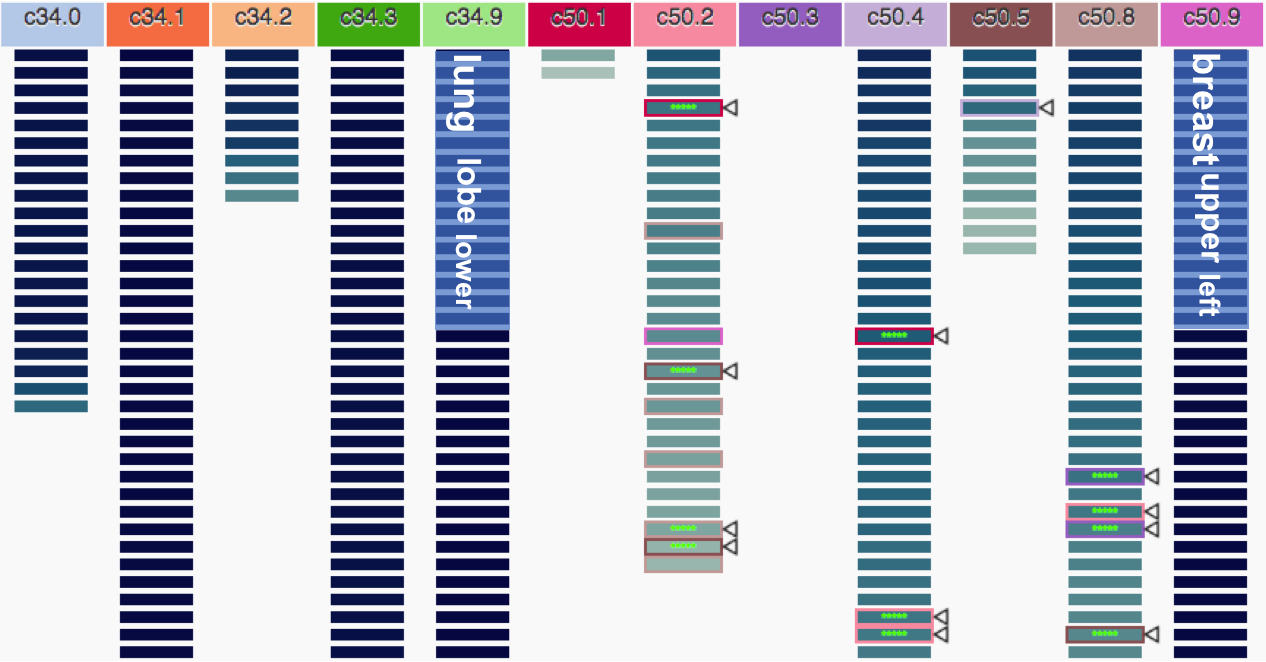
\includegraphics[width=1.0\columnwidth]{classification-view_v2}
\caption{Classification View: Samples (small narrow boxes) are visualized according to their predicted classes. The box colors represent their predicted scores. Outlined boxes are incorrectly predicted samples.
Small triangles denote the samples whose the misclassified number is more than mis-prediction threshold value.}
\label{fig:classification-view}
%\vspace{-0.8cm}
\end{figure}

\subsection{Classification View}
Our classification view is to explore classification results and to identify misclassified samples.
For each sample, neural networks usually produce predicted scores across all classes.
The class with the highest score is selected as the predicted class.
The columns in the view (Figure~\ref{fig:classification-view}) represent the classes and each column head has its class name and an unique color.
Under the heads, each narrow box corresponds a sample (a pathology report in this paper) and the boxes are lined along their predicted class columns and ordered by their scores.
For each class, the stacked boxes as a whole is a bar that is a suitable visual variable for comparing quantity (the number of samples for each class)~\cite{cleveland1984graphical}. 
A sample is selected by users, we add green markers inside the box.
Once users change the epoch using the slider control (Figure~\ref{fig:teaser} (B)) and then the classification view dynamically updates the result corresponding to the current selected epoch.

The solid boxes for each column represent samples correctly predicted while the outlined boxes represent samples incorrectly predicted.
The fill color of each box indicates the predicted score assigned to the predicted class.
The score is varied from 0 to 1 and the sum of the scores is 1.
%since the score set for a sample is a softmax output.
In other words, the boxes with the dark blue color are predicted with high confidence while the boxes with the light blue color are predicted with low confidence.
This allows to inspect the samples that are ambiguously classified\textemdash its predicted scores are evenly distributed across all classes.
In addition, the color gradient of stacked boxes as a whole shows that how confidently the model classifies the samples for the corresponding class.
It possibly suggests the directions to increase the accuracy of the model.
The outline color of a misclassified sample indicates the class which the sample is labeled as.
The misclassified samples usually have relatively low confidence as shown in Figure~\ref{fig:classification-view}.
Also, we provide a different type of visualization for the classification view as an alternative option as shown in Figure~\ref{fig:grid-mode}.
This type can handle more number of samples and is useful when we use a small size of display.

If the number of incorrect prediction for a sample is greater than the value of the mis-prediction threshold slider (Figure~\ref{fig:teaser} (C)) as epochs progress, we indicate the samples with the small triangles.
This allows to see that what samples are continuously mis-predicted during the training process.
Users can examine the samples using the detail view to find reasons for misclassification.

Also, we extract a set of words considered to be important by HAN from samples for each class and allow to display those over the column by user selection (This function is not completely implemented yet).
The font size of each word indicates its importance.
For example, we display a set of three keywords for each of the two selected columns: \textit{c34.9} and \textit{c50.9} as shown in Figure~\ref{fig:classification-view}.
We can see what are the major keywords of each class even though we have no background knowledge on the reports and classes.

\subsection{Predicted Probability Distribution View}
Our visual analytics system utilizes a standard parallel coordinate visualization to enable examining of the predicted score distributions over classes for the selected samples.
As we mentioned previously, to increase the classification accuracy, it is important to know what samples are incorrectly predicted and how their predicted scores are distributed.
%, and what classes are secondly or thirdly predicted.
We show an example case in Figure~\ref{fig:prodis}.
We select the samples that are predicted as a class (c50.4) with low confidence (Figure~\ref{fig:prodis} (A)).
The numbers of incorrect prediction of the selected samples are greater than the mis-prediction threshold value set as 10.
We can see their predicted score distributions as shown in Figure~\ref{fig:prodis} (B).
We filter the samples whose scores assigned to another class (c50.8) are over 0.3 as shown in Figure~\ref{fig:prodis} (C).
We can see that the model confuses the two classes, \textit{c50.4} and \textit{c50.8}.
This can provide an opportunity to investigate why the model cannot clearly distinguish between the two different classes.

\begin{figure}[tb]
\centering
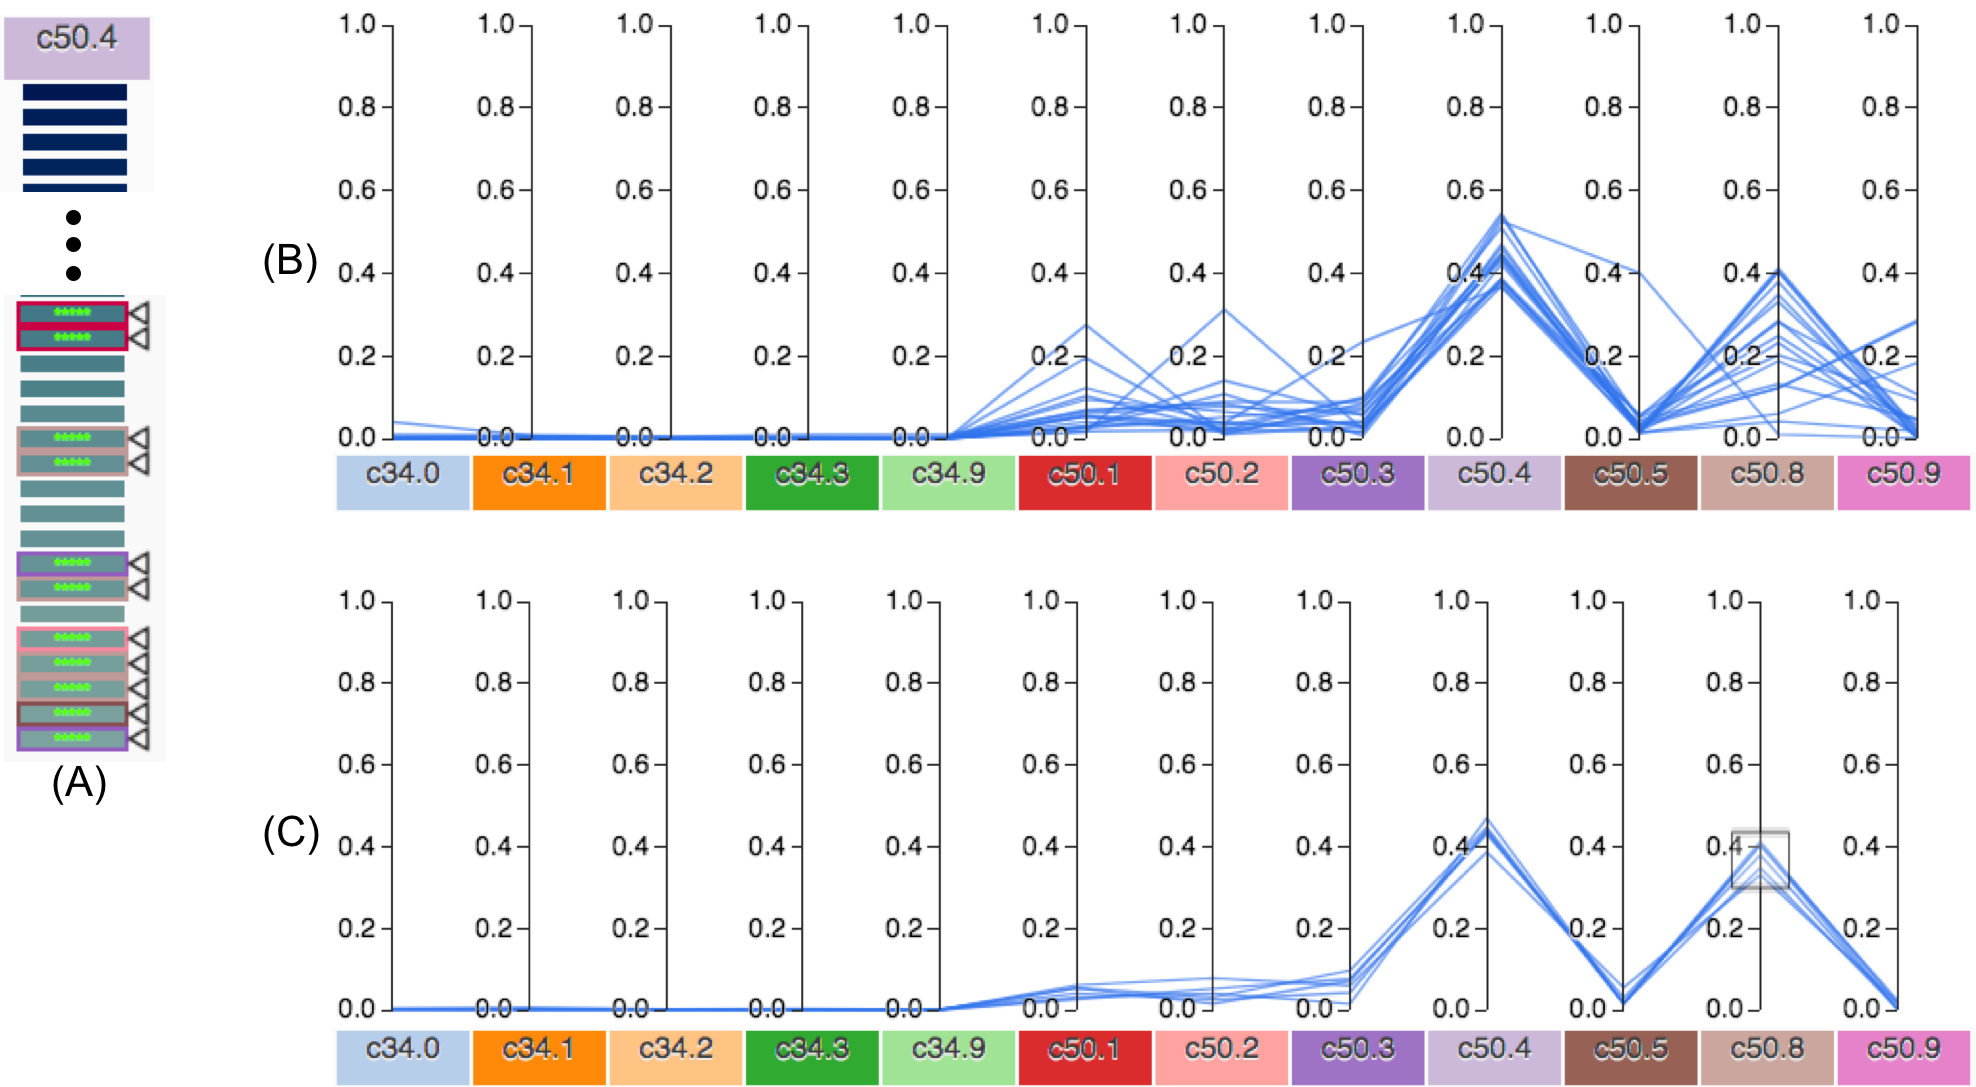
\includegraphics[width=1.0\columnwidth]{prodis_v2}
\caption{Selected samples in the class, c50.4 (A). The predicted score distributions of the selected samples (B). Filtering the samples with its score of the class, c50.8 over 0.3 (C). The model confuses the two classes: c50.4 and c50.8}
\label{fig:prodis}
%\vspace{-0.8cm}
\end{figure}

\subsection{Detail View}
Finally, our detail view visualizes the features of each sample learned by the neural networks.
An example is shown in Figure~\ref{fig:detail-view}.
We utilize the Hierarchical Attention Network (HAN) described in Section~\ref{sec:background} to extract important words and sentences from a huge volume of pathology reports and to classify the reports.
For each report, we visualize the words and the lines (sentences) with their importance in the detail view.
The dark red and dark blue colors denote highly important lines and words, respectively.
On the other hand, the light blue and red colors denote little important lines and words.
In the example view in Figure~\ref{fig:detail-view}, we can see the highlighted important words and lines which usually include the important words.
In this paper the detail view supports only a document type of data, but it is possible to visualize the learned features of other types of data.
For example, in image classification, we can highlight the learned features on an image using other feature detection techniques~\cite{zhou2016learning}.
We leave this as a future work.

















\section{Conclusion}

In conclusion, we described our visual analytics tool for understanding of classification results in Deep Neural Networks (DNNs).
Our visual components of the tool allows DNN experts to track the accuracy of their model, explore the classification results, examine the predicted score distributions of samples, and see the learned features of samples.
Eventually, our visualization helps the experts understand and diagnose the DNN model and suggest potential directions to improve the model.
This tool still has limitations in understanding inner process of DNNs and handling and visualizing a huge volume of samples.
For future work, we will investigate the ways to understand inner transactions of neurons and layers in DNNs and improve the current visual design to cover bigger size of data.




\begin{acknowledgments}
This work has been supported in part by the Joint Design of Advanced Computing Solutions for Cancer (JDACS4C) program established by the U.S. Department of Energy (DOE) and the National Cancer Institute (NCI) of the National Institutes of Health. This work was performed under the auspices of the U.S. Department of Energy by Argonne National Laboratory under Contract DE-AC02-06-CH11357, Lawrence Livermore National Laboratory under Contract DE- AC52-07NA27344, Los Alamos National Laboratory under Contract DE-AC5206NA25396, and Oak Ridge National Laboratory under Contract DE-AC05-00OR22725. This research was supported by the Exascale Computing Project (17-SC-20-SC), a collaborative effort of the U.S. Department of Energy Office of Science and the National Nuclear Security Administration.
\end{acknowledgments}

%\bibliographystyle{abbrv}
\bibliographystyle{abbrv-doi}
%\bibliographystyle{abbrv-doi-narrow}
%\bibliographystyle{abbrv-doi-hyperref}
%\bibliographystyle{abbrv-doi-hyperref-narrow}

\bibliography{template}

\begin{figure*}[tb]
\centering
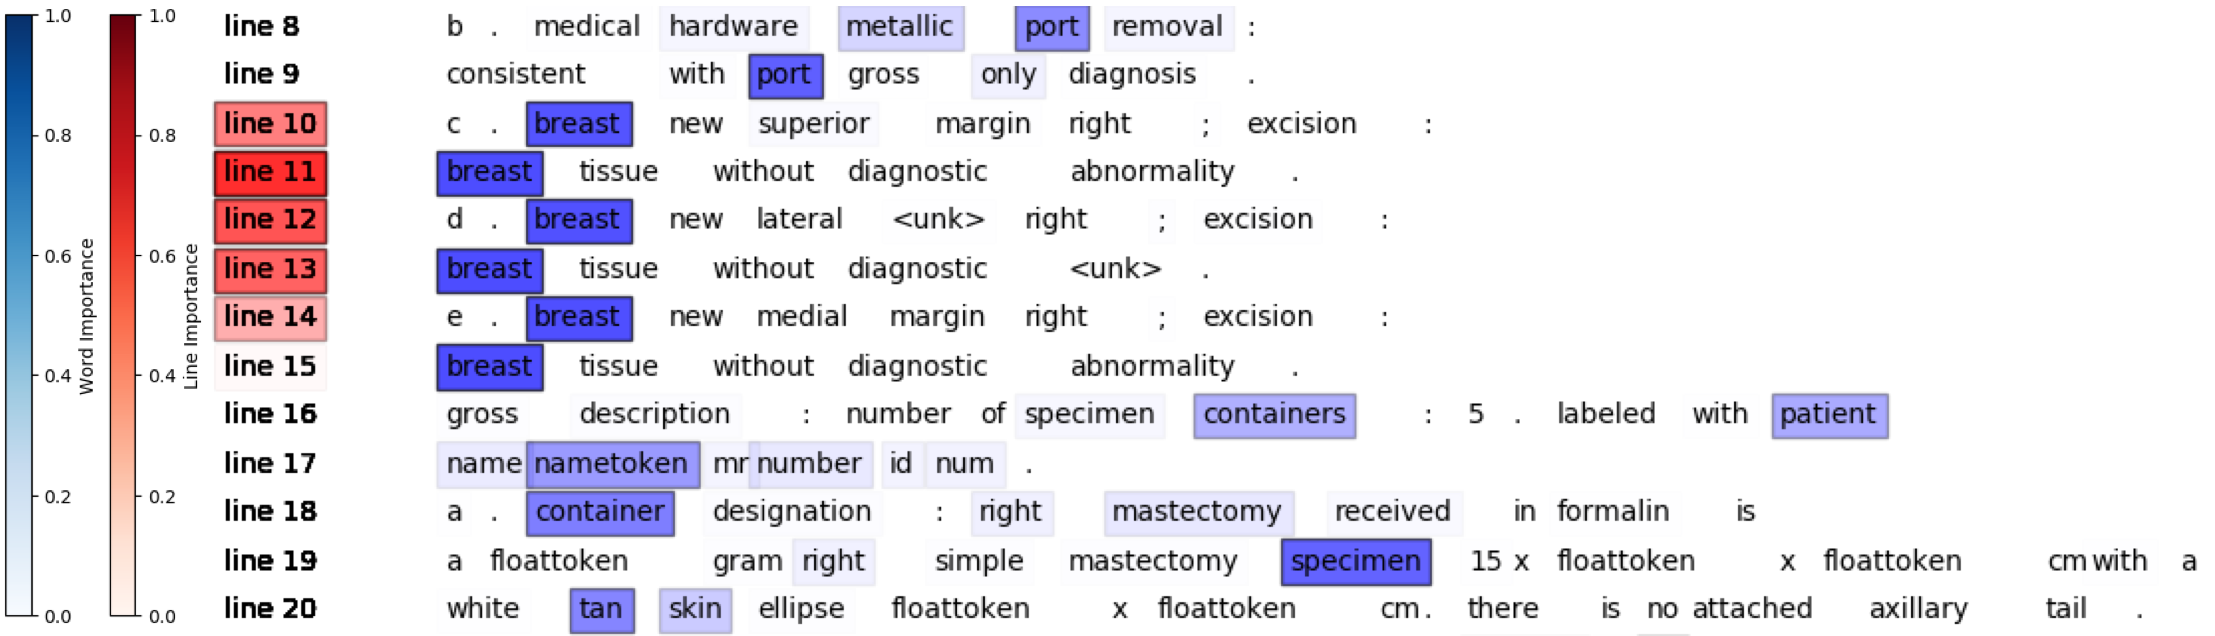
\includegraphics[width=1.0\linewidth]{doc-image}
\caption{Detail View: Visualizing important words and sentences in a pathology report.}
\label{fig:detail-view}
%\vspace{-0.8cm}
\end{figure*}


\begin{figure*}[tbh]
\centering
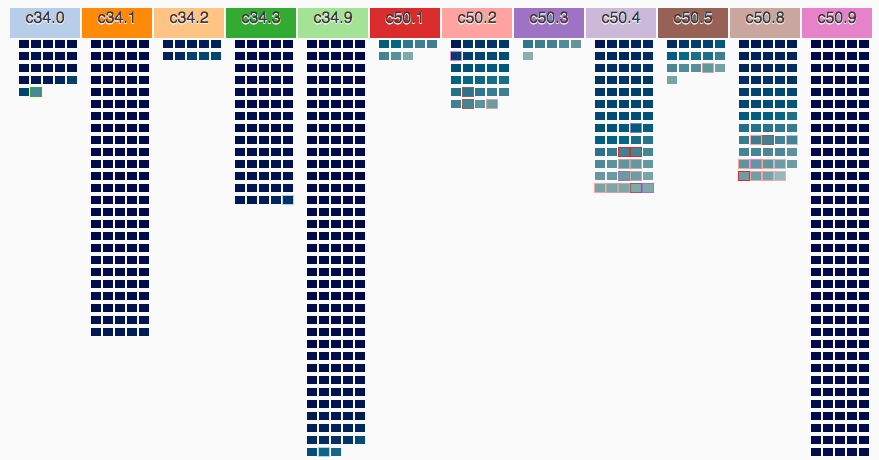
\includegraphics[width=1.0\linewidth]{grid-mode}
\caption{Grid-based classification view. This type can handle more number of samples.}
\label{fig:grid-mode}
%\vspace{-0.8cm}
\end{figure*}

\end{document}
